\documentclass{article}

\usepackage[T1]{fontenc}
\usepackage[polish]{babel}
\usepackage[utf8]{inputenc}
\usepackage{lmodern}
\selectlanguage{polish}

\title{Komunikacja Człowiek-Komputer \newline rozpoznawanie nut}
\author{kubawasik }
\date{November 2018}

\usepackage{natbib}
\usepackage{graphicx}
\usepackage{caption}
\usepackage{subcaption}

\begin{document}

\maketitle

\section{Zastosowanie}


Program służy do wykrywania nut ze zdjęcia.
Jest w stanie odnaleźć klucze (wiolinowy i basowy) oraz wypisać kolejność pojawienia się nuty, jej wysokość oraz numer pięciolinii, w której się znajduje.  

\section{Przetwarzanie}

Pierwszym krokiem, który należało wykonać było "wyłuskanie" ze zdjęcia samej kartki. 
W tym celu poszukiwaliśmy największego konturu na obrazie, który ma cztery narożniki, zakładając, że to nasza kartka. 
Aby było to możliwe, wcześniej nakładaliśmy filtr Canny. 
Kiedy już odnaleźliśmy nasze narożniki, po odpowiednim ich posortowaniu używaliśmy dla nich funkcji \textbf{cv2.getPerspectiveTransform()}
oraz \textbf{cv2.warpPerspective()}, aby odpowiednio znaleźć macierz transformacji i zastosować ją na zdjęciu. 

\begin{figure}
    \centering
    \begin{subfigure}{.5\textwidth}
        \centering
        \graphicspath{ {Resources/} }
        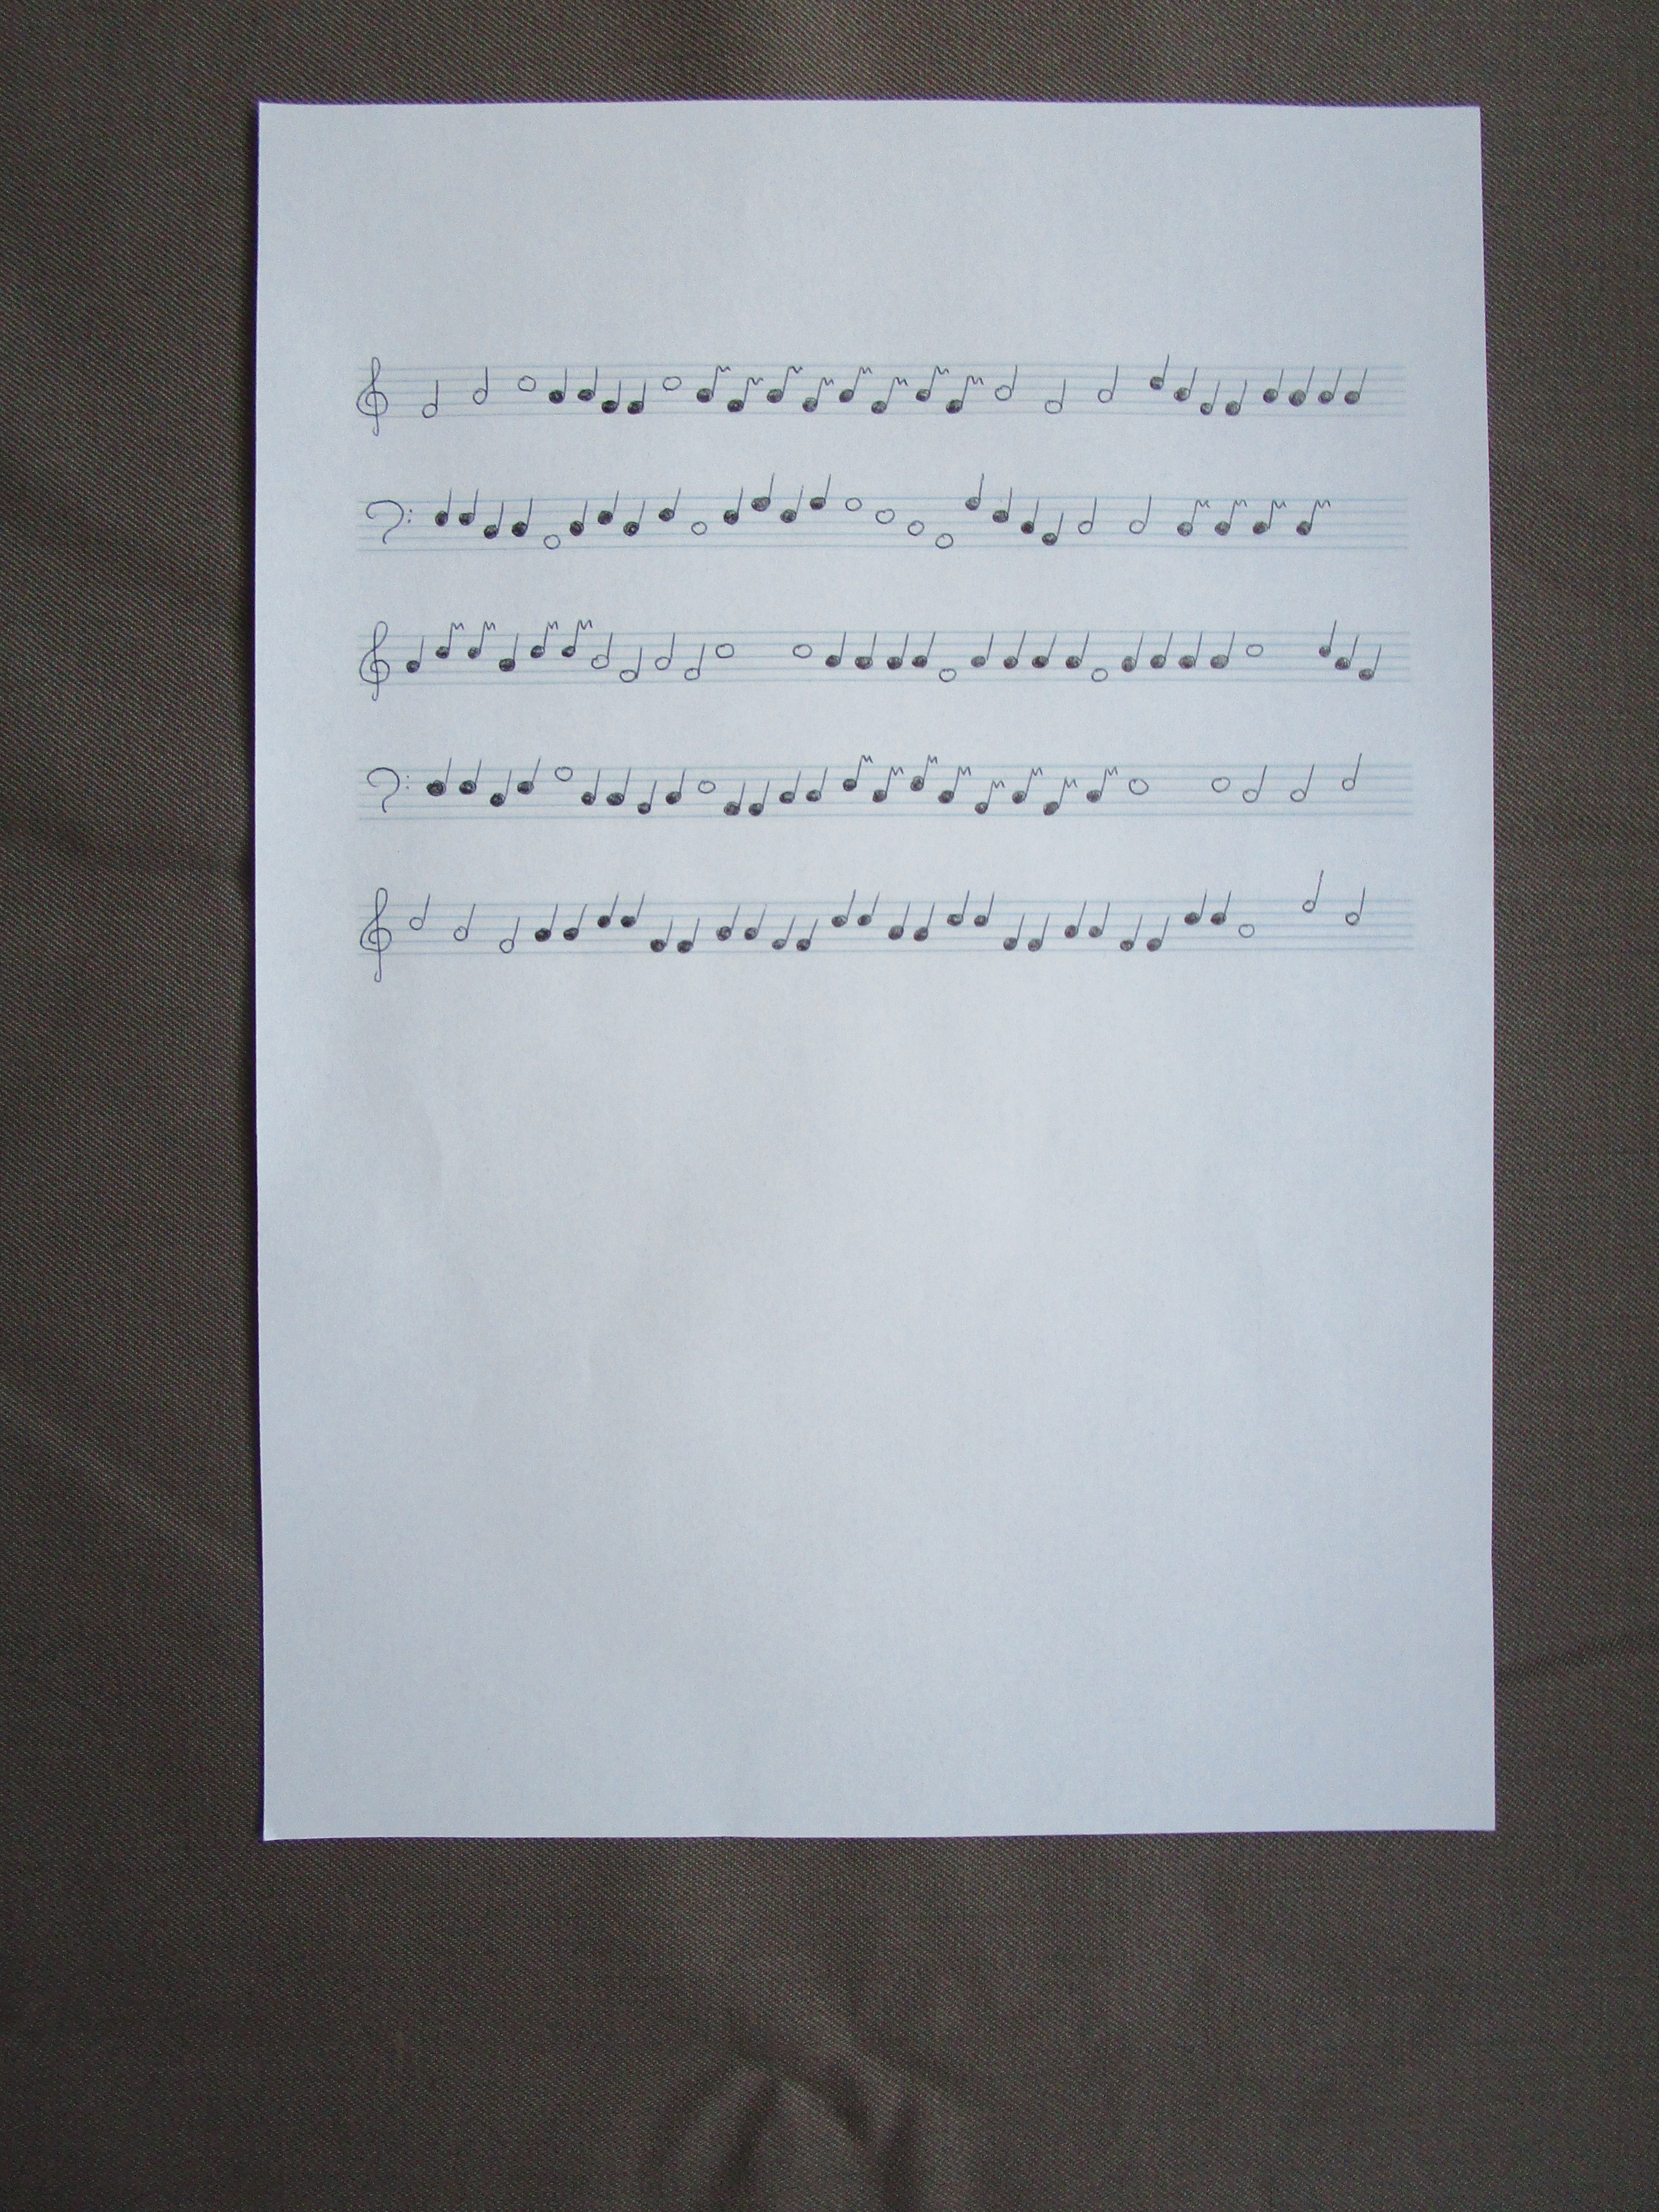
\includegraphics[width=.9\linewidth]{nutki_04.JPG}
        % \caption{A subfigure}
        \label{fig:sub1}
    \end{subfigure}%
    \begin{subfigure}{.5\textwidth}
        \centering
        \graphicspath{ {output/} }
        \includegraphics[width=.9\linewidth]{warped4_gray.jpg}
        % \caption{A subfigure}
        \label{fig:sub2}
    \end{subfigure}
    % \caption{Obraz oryginalny i po wycięciu}
    \label{fig:test}
\end{figure}
\begin{figure}
    \centering
    \begin{subfigure}{.5\textwidth}
        \centering
        \graphicspath{ {Resources/} }
        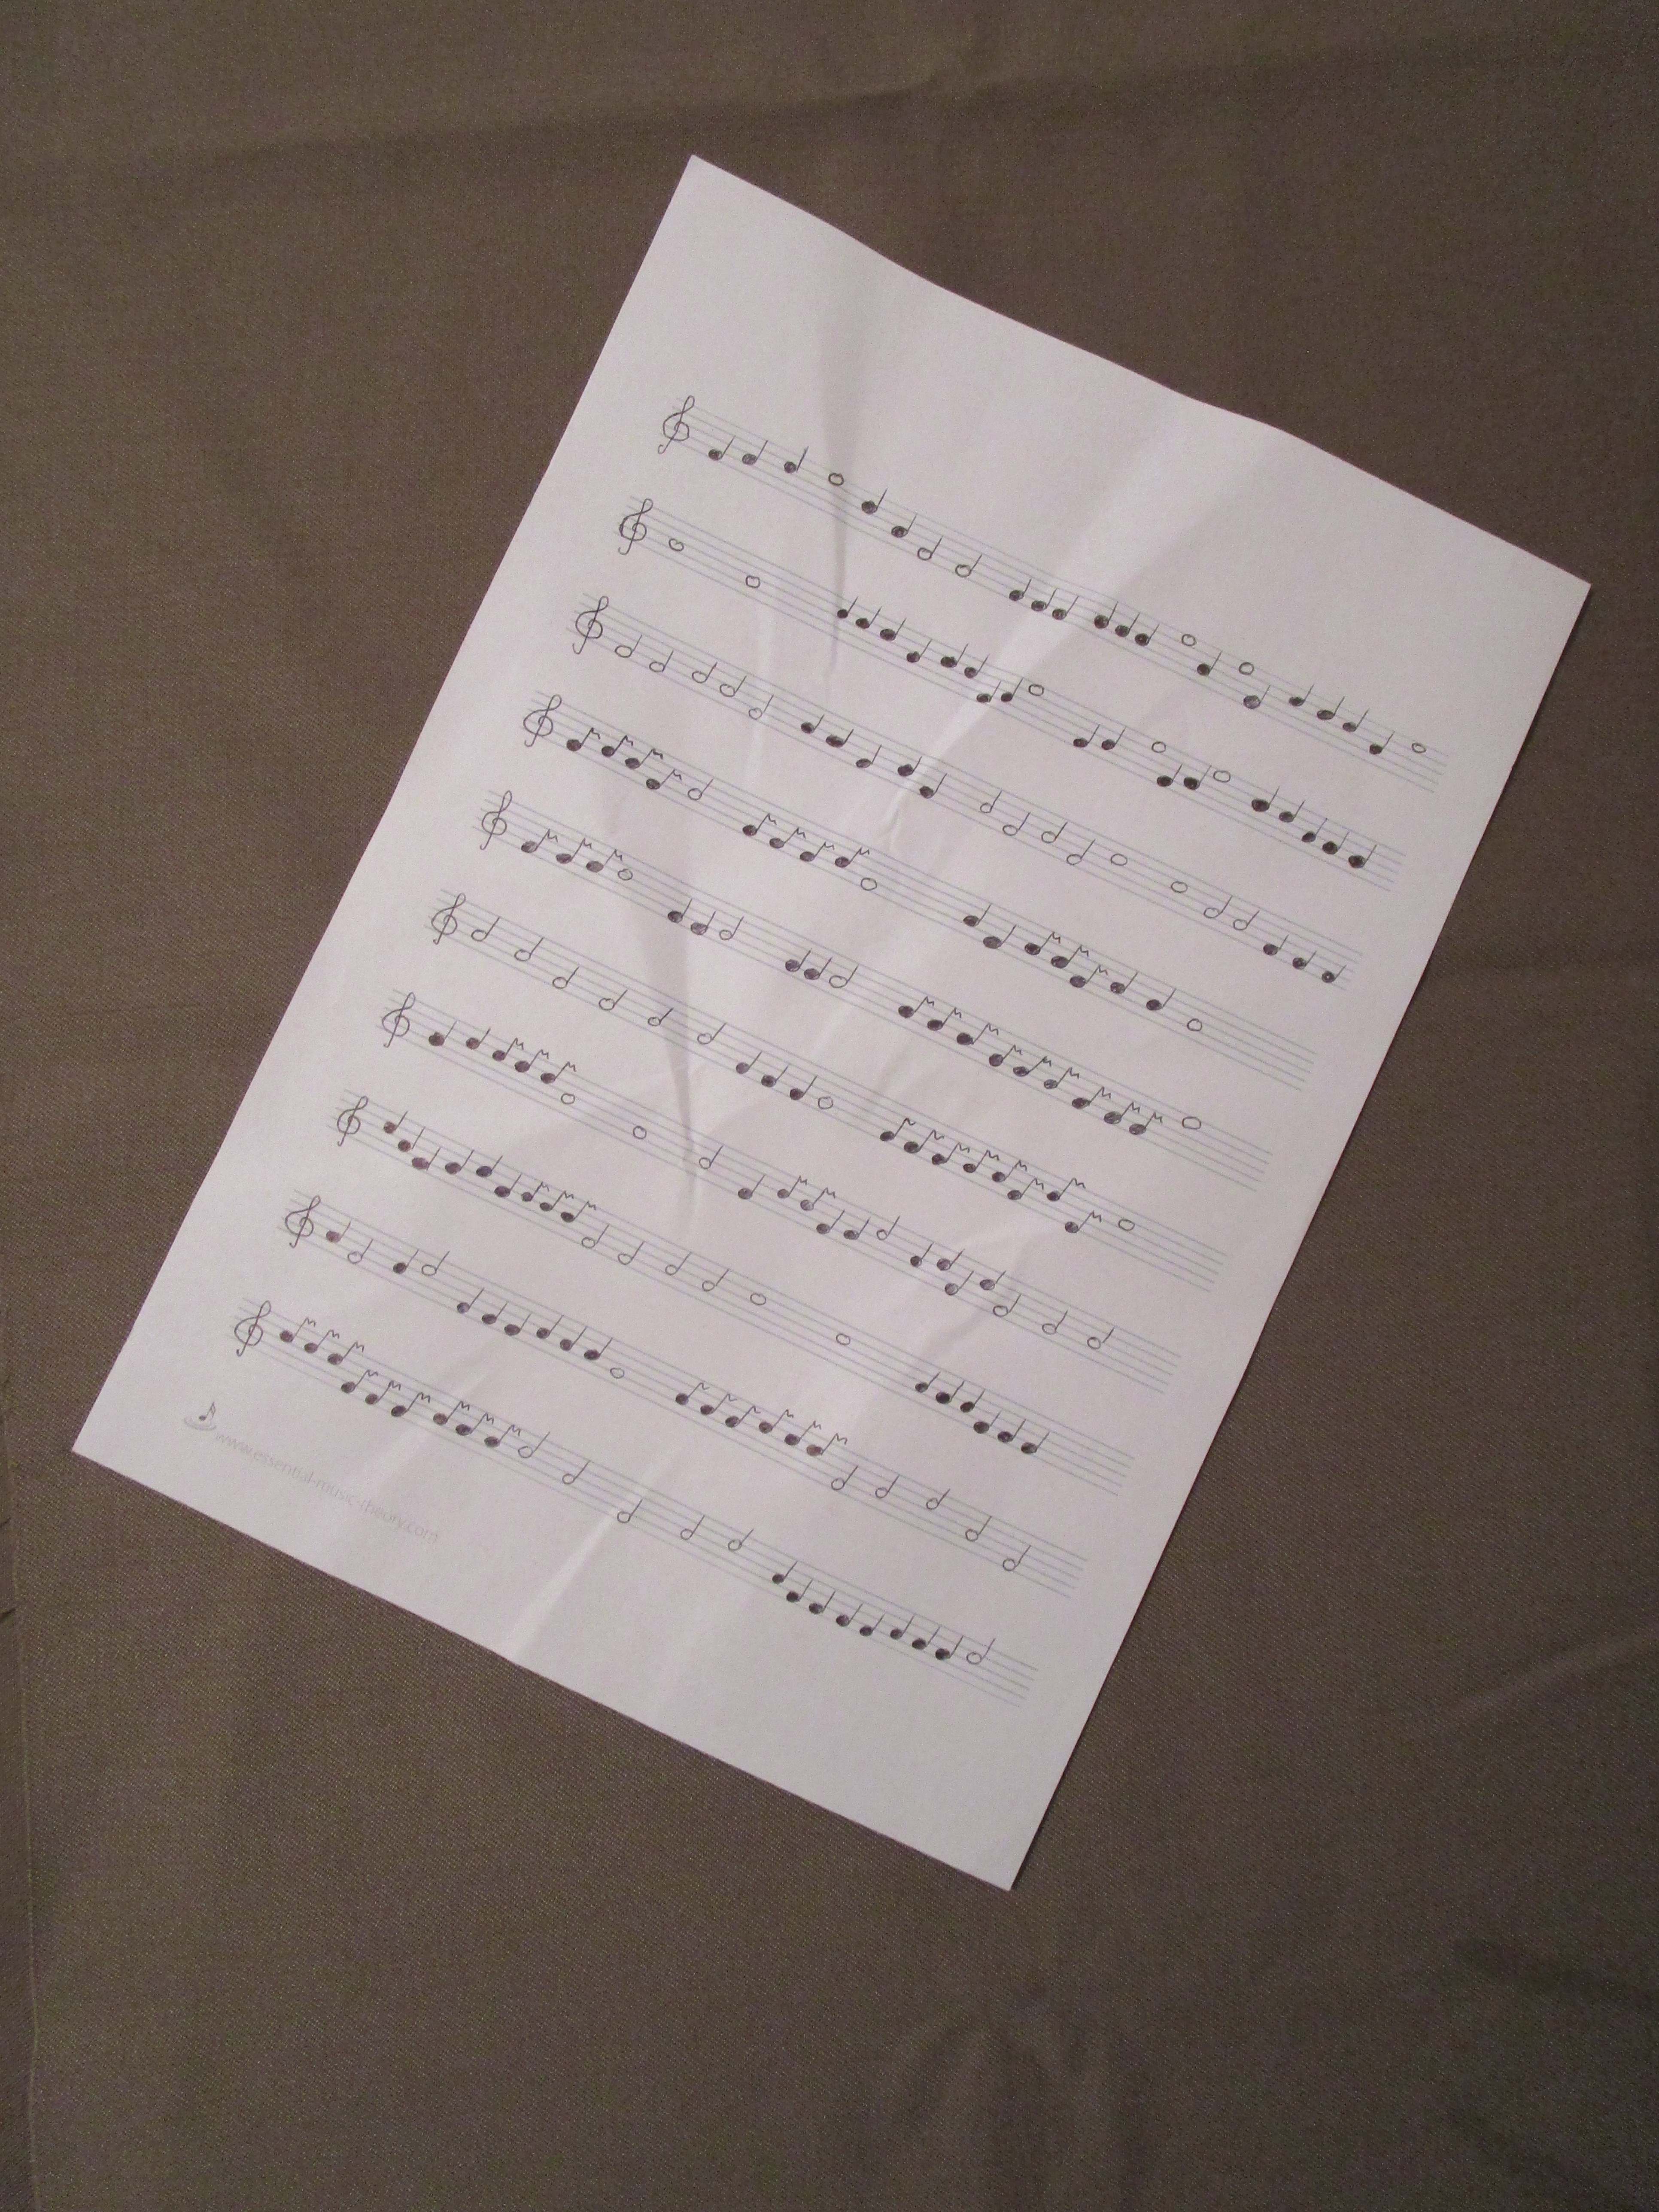
\includegraphics[width=.9\linewidth]{nutki_21.JPG}
        % \caption{A subfigure}
        \label{fig:sub1}
    \end{subfigure}%
    \begin{subfigure}{.5\textwidth}
        \centering
        \graphicspath{ {output/} }
        \includegraphics[width=.9\linewidth]{warped21_gray.jpg}
        % \caption{A subfigure}
        \label{fig:sub2}
    \end{subfigure}
    \caption{Obraz oryginalny i po wycięciu}
    \label{fig:test}
\end{figure}

% \begin{figure}[h!]
% \centering
% % \includegraphics[scale=1.7]{universe}
% \caption{The Universe}
% \label{fig:universe}
% \end{figure}
\pagebreak

Nie dla wszystkich przypadków wykrywanie kartki zadziałało - dla nierównomiernego oświetlenia wykryte kontury kartki nie były zamknięte. 
Efekt takiego wycięcia wyglądał tak:

\section{Conclusion}
``I always thought something was fundamentally wrong with the universe'' \citep{adams1995hitchhiker}

\bibliographystyle{plain}
\bibliography{references}
\end{document}
